\documentclass[a4paper,12pt]{homework}
\usepackage[slovene]{babel}
\usepackage[utf8]{inputenc}
\usepackage{graphicx}
\usepackage{amsfonts}

\setlength{\parindent}{0mm}

\newcommand{\pojem}[1]{\textsc{#1}}

\newcounter{definicija}
\newenvironment{definicija}
{
	\stepcounter{definicija}
	\begin{flushleft}
		\textbf{Definicija \arabic{definicija}: }
	}
	{
		\hfill $\square$
	\end{flushleft}
}

\newcommand{\pojem}[1]{\textsc{#1}}

\newcounter{trditev}
\newenvironment{trditev}
{
	\stepcounter{trditev}
	\begin{flushleft}
		\textbf{Trditev \arabic{trditev}: }
	}
	{
	\end{flushleft}
}

\begin{document}
	\begin{titlepage}
		\begin{center}
			
\includegraphics[scale=0.50]{logo.png}
			\vspace{4cm}
			\\
			\Huge
			\textbf{PRINCIPI RAČUNANJA ZAVAROVALNIH PREMIJ}
			\\
			\vspace{1cm}
			\Large
			Zakaj mora čista premija presegati pričakovano škodo
			\\
			\vspace{2cm}
			\large
			Neža Kržan \\
			Mentor: prof. Tomaž Košir \\
			\vspace{7cm}
			Ljubljana, \\ April 2021
		\end{center}
	\end{titlepage}
	
	\newpage
	\tableofcontents
	
	\newpage
	\section{Uvod}
	Dejavnosti zavarovalnice so lahko opisane kot vhodno-izhodni sistem, v katerem je presežek zaradi zasluženih premij in obresti ter zmanjšanje oziroma možna izguba zaradi škod in stroškov. Aktuarski vidik za izračun premije je izračunati najmanjšo premijo, ki je še vseeno dovolj velika, da pokrije terjatve in poleg tega poveča pričakovan presežek za toliko, da je portfelj stabilen.
	\\
	\\
	Predpostavimo, da zavarovalnica posluje na popolno konkurenčnem trgu in so njeni stroški dela, kapitala in poslovanja enaki nič. Zavarovalnica pozna tudi matematično upanje škodnih zahtevkov za vsako leto. Poleg tega pa je poštena, torej noče ustvariti nobenega dobička. 
	\\
	\\
	Izkaže se, da mora biti čista premija, ki jo zavarovalnica zaračuna svojim strankam višja od pričakovane škode. Sicer bo njen kapital z verjetnostjo ena v nekem končnem številu obdobij negativen in bo zavarovanica slej ko prej propadla.
	
	\newpage
	\section{Zavarovalna premija}
	Zavarovalna premija je plačilo za zavarovanje oziroma cena zavarovanja. Zvarovanec plača bruto premijo, ki se ji reče tudi kosmata premija, ta pa se deli na čisto premijo in režijski dodatek oziroma vračunan stroškek. 
	
	\section{Čista premija}
	\begin{trditev} 
		Denimo, da je škoda vsako leto porazdeljena normalno, torej $N(\mu, \sigma ^2)$. Višine škodnih zahtevkov vsako leto so med seboj neodvisne in 
		\begin{itemize}
			\item $K_n$ naj bo kapital n-tega leta,
			\item $z$ naj bo začetni kapital ob letu $0$,
			\item $\mu_i$ je pričakovana vrednost šode i-tega leta ter
			\item $X_i$ naj bo višina škodnega zahtevka v i-tem letu.
		\end{itemize}
		Potem za kapital zavarovalnice v n-tem letu velja:
		\[
		K_n = z + \sum_{i=1}^n (\mu_i - X_i).
		\]
	\end{trditev}
	Če je čista premija enaka matematičnemu upanju škodnih zahtevkov, se da pokazati, da bo zavarovalnica z verjetnostjo 1 propadla v končnem času. Zvarovalnice morajo biti nepoštene in zaračunati več od pričakovane škode, sicer bo slej kot prej gotovo propadle. Če je zavarovalnica poštena, obstaja nek $m$ večji od 0, ki predstavlja leto, ko bo kapital zavarovalnice negativen, torej
	\[
	P(\exists m > 0; K_m < 0)=1.
	\]
	
	\section{Verjetnost propada}
	V zavarovalništvu se uporablja teorija propada ali teorija tveganja, ki uporablja matematične modele za opis ranljivosti zavarovalnice za plačilno nesposobnost oziroma propad. 
	\\
	\\
	Vedno upoštevamo časovni razvoj kapitala $U(t)$ zavarovalnice. Torej ko kapital postane negativen, lahko rečemo, da pride do propada zavarovalnice. Ob predpostavki, da letna premija in postopek izplačevanja odškodnin ostaneta nespremenjena, naj $\psi(u)$ označuje verjetnost, da se propad zavarovalnice zgodi. Ta verjetnost je koristna za upravljanje, saj je pokazatelj zanesljivosti kombinacije premij in škodnega postopka zavarovalnice glede na razpoložljiv začetni kapital.
	\\
	\\
	Verjetnost propada omogoča primerjavo portfeljev, ne moremo pa ji pripisati absolutni pomen verjetnosti uničenja, saj dejansko ne predstavlja verjetnosti, da bo zavarovalnica propadla. Razlogov za to je več. Prvič lahko traja več stoletij, da se propad dejansko zgodi. Očitni posegi v proces, kot je na primer izplačilo dividend ali zvišanje premije za tveganje, so izključeni pri opredelitvi verjetnosti uničenja. 
	
	\subsection{Aproksimacija verjetnosti propada}
	Za verjetnostne porazdelitve je težko najti točno vrednost verjetnosti propada $\psi(u)$, zato potrebujemo dobre in preproste približke za verjetnost propada.
	
	\begin{enumerate}
		\item Ena izmed možnosti je, da za aprksimacijsko funkcijo vzamemo 
		\[
		\psi(u) \approx \frac{1}{1 + \theta} e^{-Ru},
		\]
		kjer je $R$ koeficient prilagoditve porazdelitve velikosti terjatev. 
		\\Ta funkcija ima pravilno vrednost za $\psi(0)$ in tudi pravilno asimptotično stopnjo nevarnosti $R$.
		\item Pri prejšni aproksimaciji lahko vzamemo tudi natančno verjetnost propada porazdeljeno eksponentno s koeficientom prilagoditve R, kar je
		\[
		\psi(u) \approx (1 - R\mu_1)e^{-Ru}.
		\]
		Na ta način je stopnja nevarnosti pravilna, vendar pa se lahko verjetnost propada pri ničli razlikuje.
		\item Če zamenjamo porazdelitev terjatev z eksponentno porazdelitvijo z enako pričakovano vrednostjo, dobimo
		\[
		\psi(u) \approx \frac{1}{1 + \theta} exp(-\frac{\theta}{1+ \theta}\frac{u}{\mu_1}).
		\]
		Za $u=0$ je približek pravilen, v splošnem pa sta leva in desna stran različni.
		\item Če $\psi(u)$ aproksimiramo z $\psi(0)e^{-ku}$, kjer je $k$ tak, da velja $\int_{0}^{\infty} \psi(u) du = \frac{\mu_2}{2\theta \mu_1}$ za aproksimacijo 
		\[
		\psi(u) \approx \frac{1}{1 + \theta} exp(\frac{-2\theta \mu_1 u}{(1 + \theta)\mu_2}).
		\]
		Če so $\frac{1}{\mu_1}$ naključne spremenljivke in je $\mu_2 = 2\mu_1^2$, potem aproksimaciji pod točko 3. in 4. vrneta pravilno verjetnost propada.
		\item Še ena možnost je aproksimacija z diskretno porazdelitvijo. 
		\item Če pa verjetnost propada aprkosimiramo z geometrijsko porazdelitvijo, nam ta omogoča uporabo Panjerjeve rekurzije, če so posamezni členi celoštevilski.
	\end{enumerate}
	
	\section{Principi računanja zavarovalnih premij}
	Princip premije je dobro definirano pravilo za izračun premije za dano tveganje, ki pa je slučajna spremenljivka. Premija vključuje tako proces tveganja kot parameter tveganja, provizije in stroški pa so izločeni iz principa premije in so obravnavani ločeno.
	
	\subsection{Izračun premije od zgoraj navzdol}
	Hans Bühlmann je opisal pristop od zgodraj navzdol za izračun premij. Pristop prikaže kako so premije povezane z merilom stabilnosti naloženim na portfelj tveganja in z zahtevami po dividendah za kapital vložene v zavarovalniško dejavnost.
	\\
	\\
	Pri tem principu si najprej ogledamo premijo, ki jo zahteva celoten portfelj. Nato upoštevamo problem pravične porazdelitve celotne premije na vse police. Za določitev najnižje letne premije pa uporabimo verjetnost propada. Rezultat je eksponentna premija, pri čemer parameter nenaklonjenosti tveganju $\alpha$  izhaja iz največje dovoljene verjetnosti propada in razpoložljivega začetnega kapitala. Ob predpostavki, da morajo biti vlagatelji začetnega kapitala nagrajeni z letno dividendo in da bi morala biti nastala premija čim nižja, torej čim bolj konkurenčna, lahko imamo optimalni začetni kapital. Pokažemo torej kako je skupna premija pošteno porazdeljena po policah in še vedno izpolnjuje naše cilje.
	
	\section{Simulacija}
	Zakaj mora čista premija presegati pričakovano škodo preverimo še na simulaciji. 
	\\
	\\
	Zamislimo si preprost scenarij, kjer imamo več zavarovalnic z isto količino začetnega kapitala. Vsaka od njih vsako leto z verjetnostjo $50 \%$ pridobi ali z verjetnostjo $50 \%$ izgubi eno enoto kapitala. Določimo začetno količino kapitala, število zavarovalnic in število let v katerih opazujemo ali kapital katere od zavarovalnic pade na 0.
	
	\subsection{Začetni model}
	V začetni simulaciji opazujemo 100 zavarovalnic ter speminjamo njihov začetni kapital ter leta opazovanja in na koncu pogledamo koliko odstotkov zavarovalnic je propadlo. 
	\\ Rezultati so predstavleni v spodnji tabeli, kjer $z$ predstavlja začetni kapital, ki narašča od $3$ do $100$, leta tečejo od $10$ do $500000$, v tabeli pa so podani tudi deleži propadlih zavarovalnic.
	
	\begin{table}[htb]
		\centering
		\caption{Deleži propadlih zavarovalnic v odvisnosti od začetnega kapitala}\vspace{2mm}
		\begin{tabular}{|c|c|c|c|c|c|c|c|c|c|c|}
			\hline
			\textbf{z} \backslash \textbf{leta} & \textbf{10} & \textbf{30} & \textbf{50} & \textbf{100} & \textbf{300} & \textbf{500} & \textbf{1000} & \textbf{5000} & \textbf{10000} & \textbf{500000} \\\hline
			\textbf{3} & 0.31 & 0.51 & 0.64 & 0.72 & 0.84 & 0.90 & 0.96 & 0.98 & 0.99 & 1 \\\hline
			\textbf{5} & 0.09 & 0.47 & 0.51 & 0.67 & 0.80 & 0.86 & 0.90 & 0.94 & 0.97 & 1 \\\hline
			\textbf{8} & 0.03 & 0.19 & 0.29 & 0.41 & 0.62 & 0.72 & 0.82 & 0.91 & 0.94 & 1 \\\hline
			\textbf{10} & 0 & 0.09 & 0.16 & 0.32 & 0.50 & 0.66 & 0.75 & 0.85 & 0.92 & 1 \\\hline
			\textbf{15} & 0 & 0.01 & 0.06 & 0.13 & 0.26 & 0.55 & 0.70 & 0.80 & 0.87 & 0.99 \\\hline
			\textbf{20} & 0 & 0 & 0.02 & 0.07 & 0.21 & 0.40 & 0.56 & 0.73 & 0.84 & 0.98 \\\hline
			\textbf{25} & 0 & 0 & 0 & 0.03 & 0.13 & 0.29 & 0.45 & 0.66 & 0.81 & 0.91 \\\hline
			\textbf{30} & 0 & 0 & 0 & 0.01 & 0.08 & 0.18 & 0.33 & 0.62 & 0.75 & 0.97 \\\hline
			\textbf{50} & 0 & 0 & 0 & 0 & 0.01 & 0.05 & 0.09 & 0.47 & 0.64 & 0.93 \\\hline
			\textbf{100} & 0 & 0 & 0 & 0 & 0 & 0 & 0.01 & 0.19 & 0.31 & 0.88 \\\hline
		\end{tabular}
		\label{tab:my_label}
	\end{table}
	
	\subsection{Začetni kapital}
	Verjetnost propada lahko zelo zmanjšamo že z majhnim povečanjem začetnega kapitala. Potrebno je gledati veliko daljše obdobje, da postane verjetnost propada blizu 1. 
	\\
	\newpage
	Na naslednjem grafu sem fiksirala dolžino obdobja na 1000 let in opazovala verjetnost propada v odvisnosti od začetnega kapitala, ki teče od 1 do 100.
	
	\begin{center}
		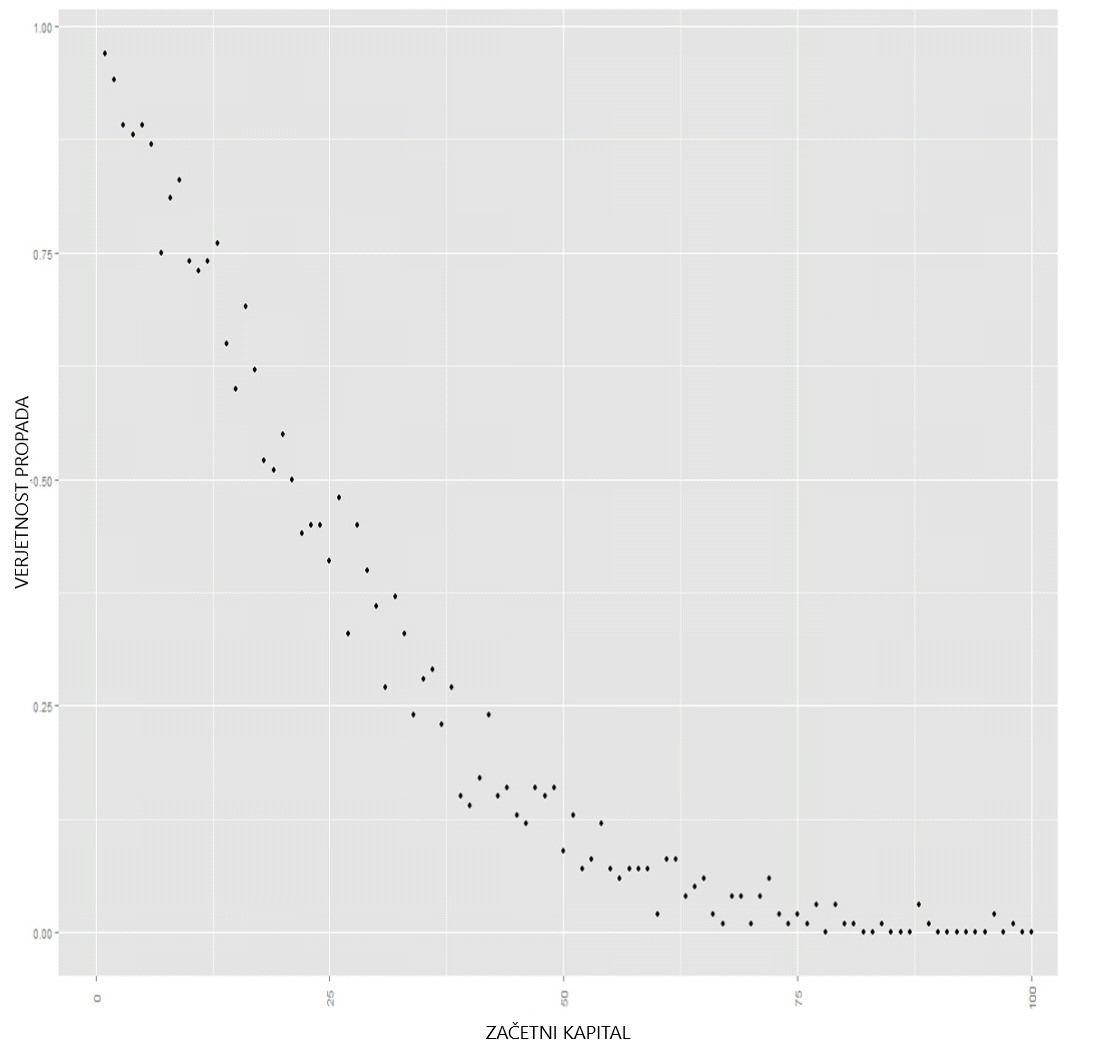
\includegraphics[scale=0.32]{graf1.jpg}  
	\end{center}
	
	\subsection{Na dolgi rok je verjetnost propada 1}
	Kljub poljubnemu povečanju začetnega kapitala se na dolgi rok ne moremo zavarovati pred propadom. Za vsak začetni kapital obstaja obdobje v katerem bo verjetnost propada limitirala proti $1$. Sicer je res potrebno pri začetnem kapitalu večjem od $100$ gledati obdobje daljše od 1000 let, vendar je kljub temu propad neizbežen. To se vidi v Tabeli 1, kjer za zelo dolga obdobja vse verjetnosti limitirajo proti $1$. Na naslednjem grafu so prikazane verjetnosti propada za zavarovalnice z začetnim kapitalom $3$, ko dolžina obdobja teče od 1 do 100 let.
	
	\begin{center}
		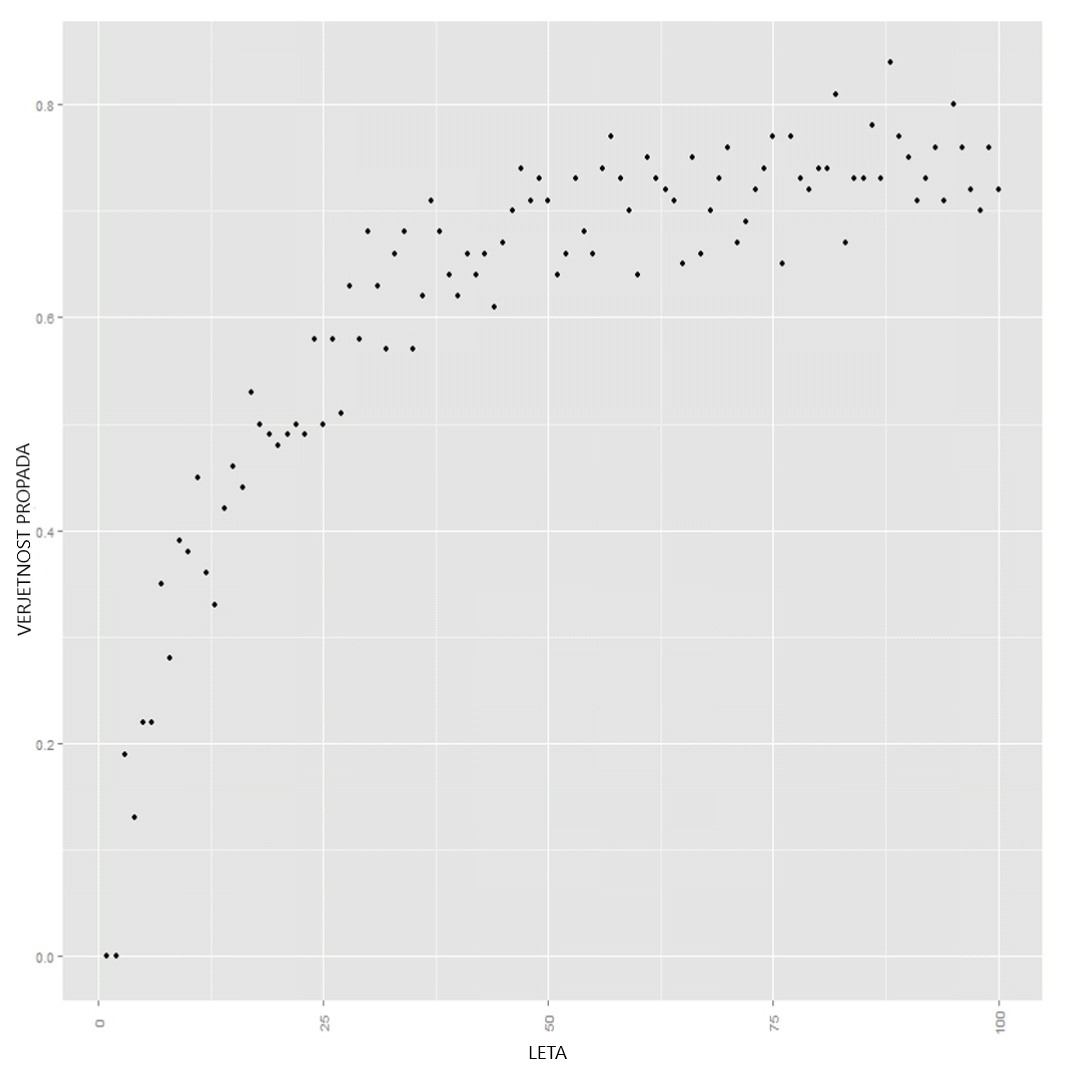
\includegraphics[scale=0.32]{graf3.jpg}  
	\end{center}
	
	\subsection{Spremenjene verjetnosti}
	Simulacijo sem spremenila tako, da bi zavarovalnica povečala čisto premijo. Verjetnost slabega stanja je še vedno $50\%$, vendar se takrat kapital zavarovalnice zmanjša za $0.5$, v dobrem stanju pa se poveča za $1.5$ enote. Sedaj se verjetnost propda zavarovalnice zmanjša skoraj na nič. Dolžina opazovanega obdobja ne vpliva na propad, saj se bo sedaj kapital zavarovalnice na daljše obdobje samo še bolj povečal. Zavarovalnica bo propadla samo v primeru, ko je njen začetni kapital manjši od $5$ enot. Takrat dejansko obstaja kakršnakoli realistična možnost propada.
	\\
	\\
	Na naslednjem grafu je kapital fiksiran na $3$ enote, obdobje opazovanja teče od $1$ do $200$ let in opazimo lahko, da je tukaj verjetnost propada skozi čas konstnatna in zelo nizka. Če bi začetni kapital povečali na $10$ enot, bi verjetnosti propada limitirale proti 0.
	
	\begin{center}
		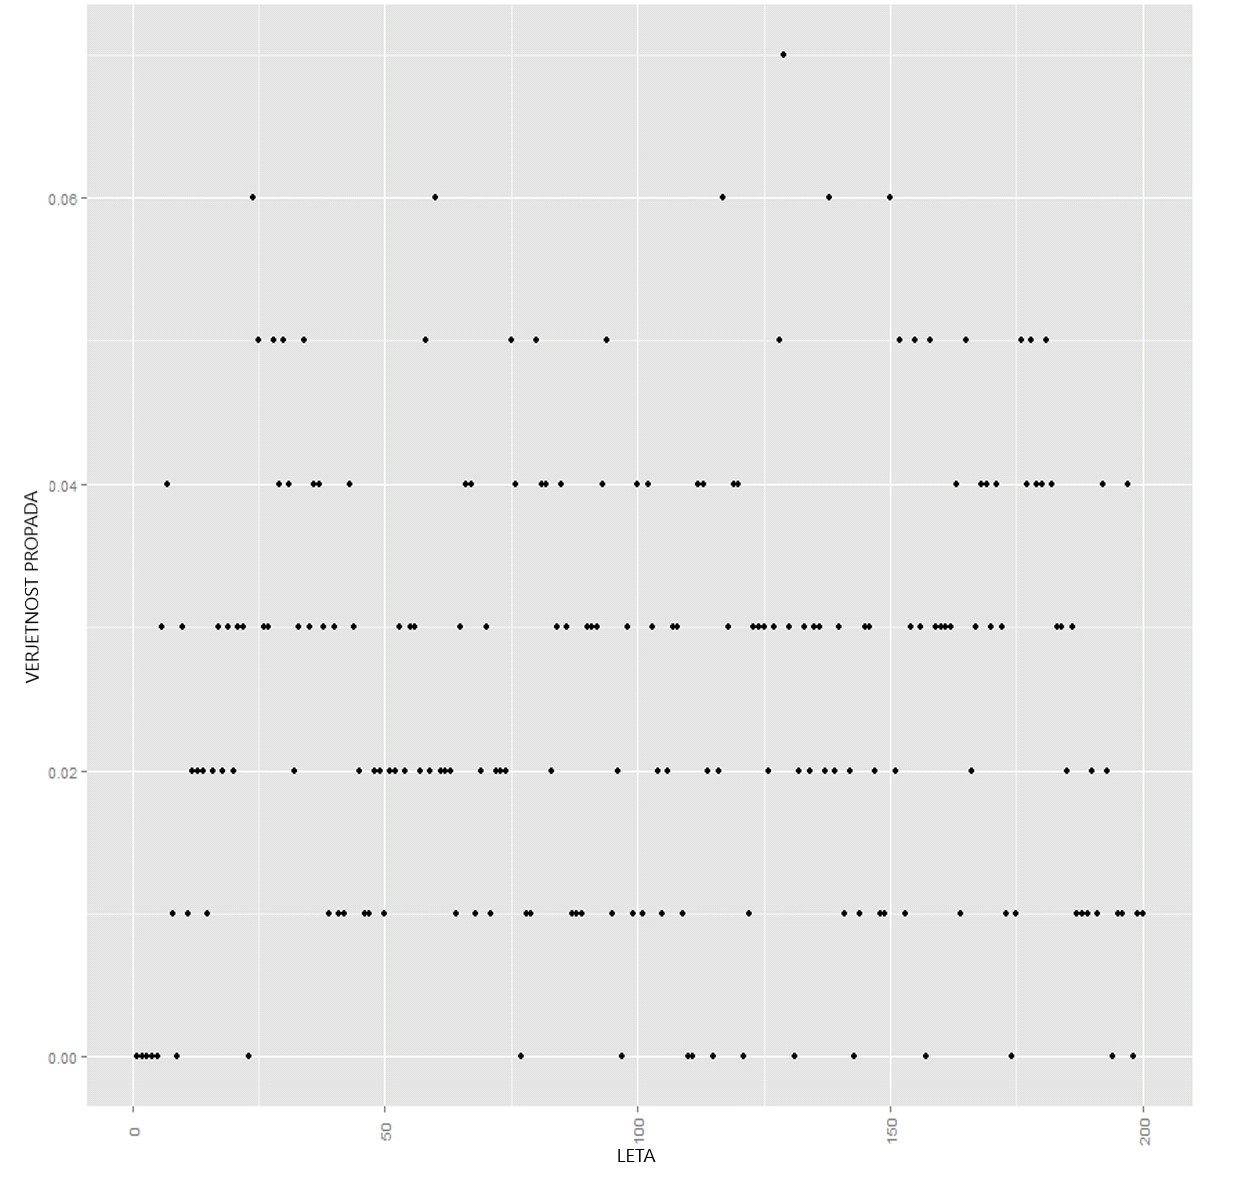
\includegraphics[scale=0.32]{graf2.jpg}  
	\end{center}
	
	\newpage
	\section{Zaključek}
	Vidimo torej, da mora čista remija presegati matematično upanje pričkovane škode, sicer bo zavarovalnica slej ko prej propadla. 
	\\
	\\V primeru nepoštene oziroma višje premije ne obstaja več neko obdobje, v katerem bo kapital zavarovalnice z gotovostjo enak $0$. Kvečejmu se skozi čas kapital veča. Propad je možen le na začetku obdobja, če je začetni kapital zavarovalnice nizek in če se zgodi veliko slabih scenarijev zapored, kar povzroči padec kapitala na $0$.
	\newpage
	\begin{thebibliography}{99}
		\bibitem{Wüthrich}
		M. V. Wüthrich. \textit{Non - Life Insurance: Mathematics and Statistics}.
		\bibitem{Schmidli}
		H. Schmidli. \textit{Lecture Notes on Risk Theory}.
		\bibitem{Kass, Goovaerts, Dhaene, Denuit} 
		R. Kass, M. Goovaerts, J. Dhaene, M. Denuit. \textit{Modern Actuarial Risk Theory}. Kluwer Academic Publ. 2001.
	\end{thebibliography}
	
\end{document}